\documentclass[11pt]{article}

\usepackage{iftex}
\ifPDFTeX
  \usepackage[utf8]{inputenc}
  \usepackage[T1]{fontenc}
  \usepackage{lmodern}
\else
  \usepackage{fontspec}
\fi
\usepackage{amsmath}
\usepackage[spanish,es-noindentfirst,es-tabla]{babel}
\usepackage{graphicx}
\usepackage{booktabs}
\usepackage{tabularx}
\usepackage{array}
\usepackage{geometry}
\usepackage[table]{xcolor}
\usepackage{titlesec}
\usepackage{caption}
\usepackage{float}
\usepackage{enumitem}
\usepackage{fancyhdr}
\usepackage{pdflscape}
\usepackage[hidelinks]{hyperref}

\geometry{a4paper, top=2.4cm, bottom=2.6cm, left=2.4cm, right=2.4cm}

\definecolor{usblue}{RGB}{23,55,94}
\definecolor{usaccent}{RGB}{0,124,146}
\definecolor{usgrey}{RGB}{90,100,110}
\definecolor{tablehead}{RGB}{23,55,94}
\definecolor{tablerow}{RGB}{238,242,246}

\hypersetup{colorlinks=true, linkcolor=usblue, urlcolor=usaccent}

\titleformat{\section}{\Large\bfseries\color{usblue}}{\thesection}{0.6em}{}
\titleformat{\subsection}{\large\bfseries\color{usaccent}}{\thesubsection}{0.6em}{}
\titleformat{\subsubsection}{\normalsize\bfseries\color{usgrey}}{\thesubsubsection}{0.6em}{}

\captionsetup{font=small, labelfont={bf,color=usblue}}
\renewcommand{\arraystretch}{1.2}
\setlength{\tabcolsep}{5pt}
\setlist{itemsep=2pt, topsep=4pt}

\pagestyle{fancy}
\fancyhf{}
\fancyhead[L]{\small\color{usgrey} UrbanSafe AI --- Informe final}
\fancyhead[R]{\small\color{usgrey} DS-3022 · UTEC · 2026-II}
\fancyfoot[C]{\small\thepage}
\renewcommand{\headrulewidth}{0.4pt}

\newcommand{\code}[1]{\texttt{#1}}
\newcommand{\hrow}{\rowcolor{tablehead}\color{white}\bfseries}

\begin{document}
\renewcommand{\%}{\char37 }

%======================================================================
\begin{titlepage}
\centering

\includegraphics[width=6.5cm]{img/utec.png}\\[0.3cm]
{\color{usblue}\rule{\textwidth}{2pt}}\\[0.6cm]
{\Huge\bfseries\color{usblue} UrbanSafe AI}\\[0.35cm]
{\LARGE Ecosistema de Movilidad Predictiva y Segura}\\[0.25cm]
{\large\color{usgrey} Informe final del Producto de Datos}\\[2.1cm]

\begin{minipage}{0.85\textwidth}
\centering
{\bfseries Curso:} Desarrollo de Productos de Datos (DS-3022) --- UTEC\\[2pt]
{\bfseries Ciclo:} 2026-II\\[2pt]
{\bfseries Profesores:} Germain Garcia-Zanabria y Dominguez Bautista, Carlos Abel\\[8pt]
{\bfseries Equipo:}\\[4pt]
\begin{tabular}{@{}l@{}}
Elmer Jose Manuel Villegas Suarez (100\%)\\
Alessandro Facundo Freed Monzón Gallegos (100\%)\\
Juan David Velo Poma (100\%)
\end{tabular}
\end{minipage}

\vfill

\begin{tabular}{@{}ll@{}}
\textbf{Aplicación web:} & \url{https://dpd-project.vercel.app}\\
\textbf{API REST:} & \url{https://urbansafe-api.onrender.com/api/health}\\
\textbf{Repositorio:} & \url{https://github.com/EV081/DPD_project}\\
\textbf{Video demo:} & \textit{[enlace pendiente: completar tras subir el video]}\\
\end{tabular}

\vspace{1cm}
{\color{usblue}\rule{\textwidth}{2pt}}
\end{titlepage}

\tableofcontents
\newpage

%======================================================================
\section{Resumen}

En el transporte público de Lima (Metro Línea 1, Metropolitano con sus alimentadores y Corredores
Complementarios) el usuario no sabe cuánto falta para la próxima unidad ni qué tan llena viene, y
tampoco qué calles conviene evitar al caminar hacia la estación. \textbf{UrbanSafe AI} es una
aplicación web que responde dos preguntas:

\begin{itemize}
  \item \textbf{Eje 1 --- ¿subo a la próxima unidad?} Pronostica la demanda por hora (LightGBM),
        reconstruye la carga a bordo con una matriz origen-destino (Furness y gravedad, Ortúzar y
        Willumsen) y recomienda \emph{abordar}, \emph{esperar el siguiente} o \emph{cambiar de
        paradero}.
  \item \textbf{Eje 2 --- ¿por dónde camino?} Estima un riesgo por calle a partir de denuncias
        policiales (LightGBM Poisson) y calcula la ruta peatonal que minimiza
        $\text{largo}\times(1+\lambda\cdot\text{riesgo})$ en el entorno de $\sim$10 minutos de cada
        acceso.
\end{itemize}

\textbf{Resultados principales (test fuera de muestra).} El pronóstico de demanda logra WMAPE de
0,100 a 0,115 en Metro L1, troncal y corredores (baseline de media de 4 semanas: 0,126 a 0,167). La
clase de aforo que ve el usuario alcanza F1-macro de 0,86 en Metro L1 y 0,93 en el troncal, pero
\textbf{no cumple} el umbral de F1-macro del requerimiento RNF-01 en corredores (0,66) ni en
alimentadores (0,54) (la causa se explica en la sección~\ref{sec:f1}, más adelante). En el Eje 2, la ruta segura evita un 43,8\,\% de las denuncias
(IC 95\,\%: 38,6--50,2) con un desvío medio de 8,7\,\% de distancia (enero--agosto de 2024).

\textbf{Estado.} El producto está desplegado (Vercel + Render + Supabase), con 217 pruebas
automáticas y datos y modelos versionados. Las limitaciones (subregistro de denuncias, ausencia de
datos de bajadas, cobertura de datos hasta 2025) se declaran en la sección~\ref{sec:limit}.

%======================================================================
\section{Problema y propuesta de valor}

Los datos de la ATU solo registran \emph{subidas} (validaciones de tarjeta): no hay bajadas, GPS ni
ocupación real. Aun así, el pasajero necesita decidir en segundos si esperar o abordar. La propuesta
de valor es convertir esas validaciones históricas en una recomendación accionable y
\emph{explicada}: ocupación (\emph{Asientos}, \emph{De pie}, \emph{Saturado}), espera estimada y
probabilidad de no poder subir.

Además de la consulta en la estación, el Eje 1 incluye un \textbf{simulador} aparte: si el usuario ya conoce el paradero y el servicio que quiere usar (Metro L1, Metropolitano, corredores o alimentadores), elige un día y una hora y la app le muestra qué opción conviene tomar: ocupación y espera por hora, recomendación y plan de salida, con descarga del resultado en CSV. Para días posteriores a 2025 usa el día homólogo.

Como segundo plus, la primera y última milla se aborda con una ruta peatonal que equilibra distancia
y exposición a denuncias registradas. El producto es sobrio y de estilo familiar (referencias:
Uber, Cabify, inDrive), mobile-first, en español.

El Data Product Canvas final, con los nueve cuadros de la plantilla del curso, está en el anexo~\ref{anx:canvas}.

\subsection{Usuarios y stakeholders}

\begin{table}[H]
\centering\small
\begin{tabularx}{\textwidth}{@{}lXl@{}}
\toprule
\rowcolor{tablehead} \textcolor{white}{\bfseries Actor} & \textcolor{white}{\bfseries Interés} & \textcolor{white}{\bfseries Rol} \\
\midrule
Pasajeros y peatones & Conocer aforo y espera; caminar por calles con menos denuncias & Primario \\
\rowcolor{tablerow} Familiares y red de apoyo & Tranquilidad sobre tramos peatonales & Indirecto \\
ATU / Protransporte & Proveen datos; visibilidad de saturación & Aliado \\
\rowcolor{tablerow} Municipalidades, serenazgo & Identificar tramos críticos para patrullaje & Operativo \\
Operadores de bus & Menos aglomeración en estaciones & Indirecto \\
\bottomrule
\end{tabularx}
\caption{Mapa de stakeholders (resumen de la especificación de requerimientos).}
\end{table}

%======================================================================
\section{Datos}

\begin{table}[H]
\centering\small
\begin{tabularx}{\textwidth}{@{}p{3.6cm}Xp{3.3cm}@{}}
\toprule
\rowcolor{tablehead} \textcolor{white}{\bfseries Fuente} & \textcolor{white}{\bfseries Contenido} & \textcolor{white}{\bfseries Uso} \\
\midrule
ATU: validaciones 2025 (acceso a la información pública) & Subidas horarias: Metro L1 (26 estaciones), Metropolitano troncal (45), corredores (12 rutas, $\sim$900 paraderos), alimentadores (23 rutas) & Eje 1: entrenamiento y evaluación \\
\rowcolor{tablerow} ATU: rutas, servicios y paraderos & Catálogo oficial de líneas, trazados y paraderos (incluye fichas de horarios) & Eje 1: red, O-D y oferta \\
metrolima.info & Frecuencia aproximada de paso de cada bus y horarios del Metro de Lima & Eje 1: oferta, ETA y ocupación \\
Denuncias SIDPOL (MININTER) & 2\,594\,332 denuncias únicas de Lima y Callao & Eje 2: riesgo por calle \\
\rowcolor{tablerow} OpenStreetMap & Grafo peatonal (188\,893 segmentos) y puntos de interés & Eje 2: red de calles \\
TomTom Traffic, LocationIQ & Tráfico en vivo y autocompletado (opcionales) & Ajuste de ETA, búsqueda \\
\bottomrule
\end{tabularx}
\caption{Fuentes de datos del producto.}
\end{table}

Las etapas S05--S07 usaron datos de TransMilenio (Bogotá) como proxy mientras llegaban los datos de
la ATU; desde la S08 todo el proyecto usa datos reales de Lima.

\subsection{Preparación}

\textbf{Eje 1.} El pipeline (\code{deliveries/week10}) descarga, limpia y carga los datos ATU en
PostgreSQL; se construyen series horarias por sistema y los modelos se serializan con manifiesto
SHA-256 (v1.3.0). Para fechas de 2026 se usa el \emph{día homólogo} de 2025 y la API lo declara en
la respuesta.

\textbf{Eje 2.} El EDA de denuncias (\code{deliveries/week12/docs/EDA\_Eje2.md}) encontró que
28,3\,\% de las filas tienen la coordenada forzada al centroide de la comisaría (un valor nulo
disfrazado). La falta de coordenada no es aleatoria (depende de la comisaría; AUC 0,928 con comisaría
frente a 0,602 solo con el año), por lo que se trata como MAR: no se imputan ubicaciones y se
pondera por cobertura (tope 4). Los datos desde septiembre de 2024 se excluyen (menos de la mitad de
coordenadas utilizables). Los datos pesados no se versionan; la adquisición está documentada.

%======================================================================
\section{Requerimientos}

La especificación completa está en \code{deliveries/week15/Requirements.md}. La
tabla~\ref{tab:req} contrasta los requerimientos no funcionales y criterios de aceptación con lo
logrado.

\begin{table}[H]
\centering\small
\begin{tabularx}{\textwidth}{@{}p{1.5cm}Xp{4.6cm}@{}}
\toprule
\rowcolor{tablehead} \textcolor{white}{\bfseries Código} & \textcolor{white}{\bfseries Requisito} & \textcolor{white}{\bfseries Estado y evidencia} \\
\midrule
RNF-01 & Accuracy $\ge 0{,}75$ y F1-macro $\ge 0{,}72$ del aforo & \textbf{Parcial.} Cumple en Metro L1 y troncal; accuracy cumple en los cuatro sistemas, F1-macro no en corredores (0,66) ni alimentadores (0,54) \\
\rowcolor{tablerow} AC-03 & Recomendación correcta $\ge 80\,\%$ & \textbf{Cumple:} 96,8--99,8\,\% por sistema (pero solo el troncal supera claramente a «siempre abordar», 89,4\,\%) \\
AC-04 / RNF-02 & P95 de latencia $\le 2$ s & \textbf{Cumple en caliente} (prueba \code{test\_latencia}); el primer pedido tras inactividad tarda $\sim$50 s por el plan gratuito de Render \\
\rowcolor{tablerow} AC-05 & Ruta segura con menor riesgo que la más corta & \textbf{Cumple en promedio:} $-43{,}8\,\%$ de denuncias realizadas; no se midió el porcentaje de pares con menor riesgo \\
RNF-03 & Disponibilidad $\ge 99\,\%$ & \textbf{No garantizada} (plan gratuito de Render) \\
\rowcolor{tablerow} RNF-05 & Privacidad (Ley 29733) & Reportes nunca se exponen de forma individual; sin geolocalización continua \\
AC-06 & Usabilidad: $\ge 60\,\%$ declara menor espera percibida & \textbf{Parcial:} prueba de campo informal con un usuario real; sin encuesta formal \\
\bottomrule
\end{tabularx}
\caption{Cumplimiento de requerimientos no funcionales y criterios de aceptación.}
\label{tab:req}
\end{table}

%======================================================================
\section{Enfoque analítico}

\subsection{Eje 1: demanda, ocupación y recomendación}

\begin{enumerate}
  \item \textbf{Pronóstico de demanda.} LightGBM por sistema predice las subidas horarias de cada
        estación (o ruta y sentido en alimentadores). Baselines: media de 4 semanas y modelos por
        ruta. Se evaluó también un ensemble con Chronos-2, descartado por no superar a LightGBM y
        por requerir \code{torch}, que no cabe en la memoria del servidor.
  \item \textbf{Matriz origen-destino.} Como no existen bajadas, se estiman por \emph{viaje de
        retorno} (quien baja en $j$ por la mañana vuelve a subir en $j$ por la tarde) y se balancea
        con Furness (gravedad doblemente acotada; acotada a orígenes en corredores). Con ello se
        obtiene la carga por tramo y sentido.
  \item \textbf{Ocupación y ETA.} Con la oferta publicada (horarios y flota) se obtienen pasajeros
        por vehículo, la clase de aforo y la espera.
  \item \textbf{Recomendación.} Costo generalizado
        $2\cdot\text{caminata}+2\cdot\text{espera}+m_h\cdot\text{tiempo a bordo}$ con el
        multiplicador de hacinamiento $m_h$ de Whelan y Crockett (sentado 1,00--1,63; de pie
        1,53--2,04). «Esperar el siguiente» si $P(\text{llega lleno})\ge 0{,}5$; «cambiar de
        paradero» si uno anterior ($\le 600$ m) ahorra $\ge 3$ minutos equivalentes.
\end{enumerate}

\subsection{Eje 2: riesgo por calle y ruta segura}

\begin{itemize}
  \item \textbf{Zona:} 800 m caminando (10 min) alrededor de 1\,775 accesos (26 estaciones de
        Metro L1, 44 del Metropolitano, 993 paraderos de corredores, 712 de alimentadores): 146\,607
        segmentos (7\,012 km).
  \item \textbf{Modelo:} LightGBM con objetivo Poisson y offset de exposición, a nivel segmento
        $\times$ año, con \emph{features} solo del pasado (tasas históricas, decaimiento, calles
        vecinas, largo, tipo de vía, POIs). No se usan variables socioeconómicas ni de «calidad de
        vida» del barrio.
  \item \textbf{Ruteo:} Dijkstra sobre el costo $\text{largo}\times(1+\lambda\cdot\text{riesgo})$
        con riesgo en $[0,1]$ (\code{scipy.sparse.csgraph}); $\lambda=12$ elegido por regla fijada
        antes de mirar el test (desvío medio $\le 15\,\%$, p90 $\le 30\,\%$). Los reportes de
        usuarios (acoso, seguimiento, robo) recalibran el riesgo de forma acotada.
\end{itemize}

%======================================================================
\section{Diseño del producto y arquitectura}

\begin{figure}[H]
\centering
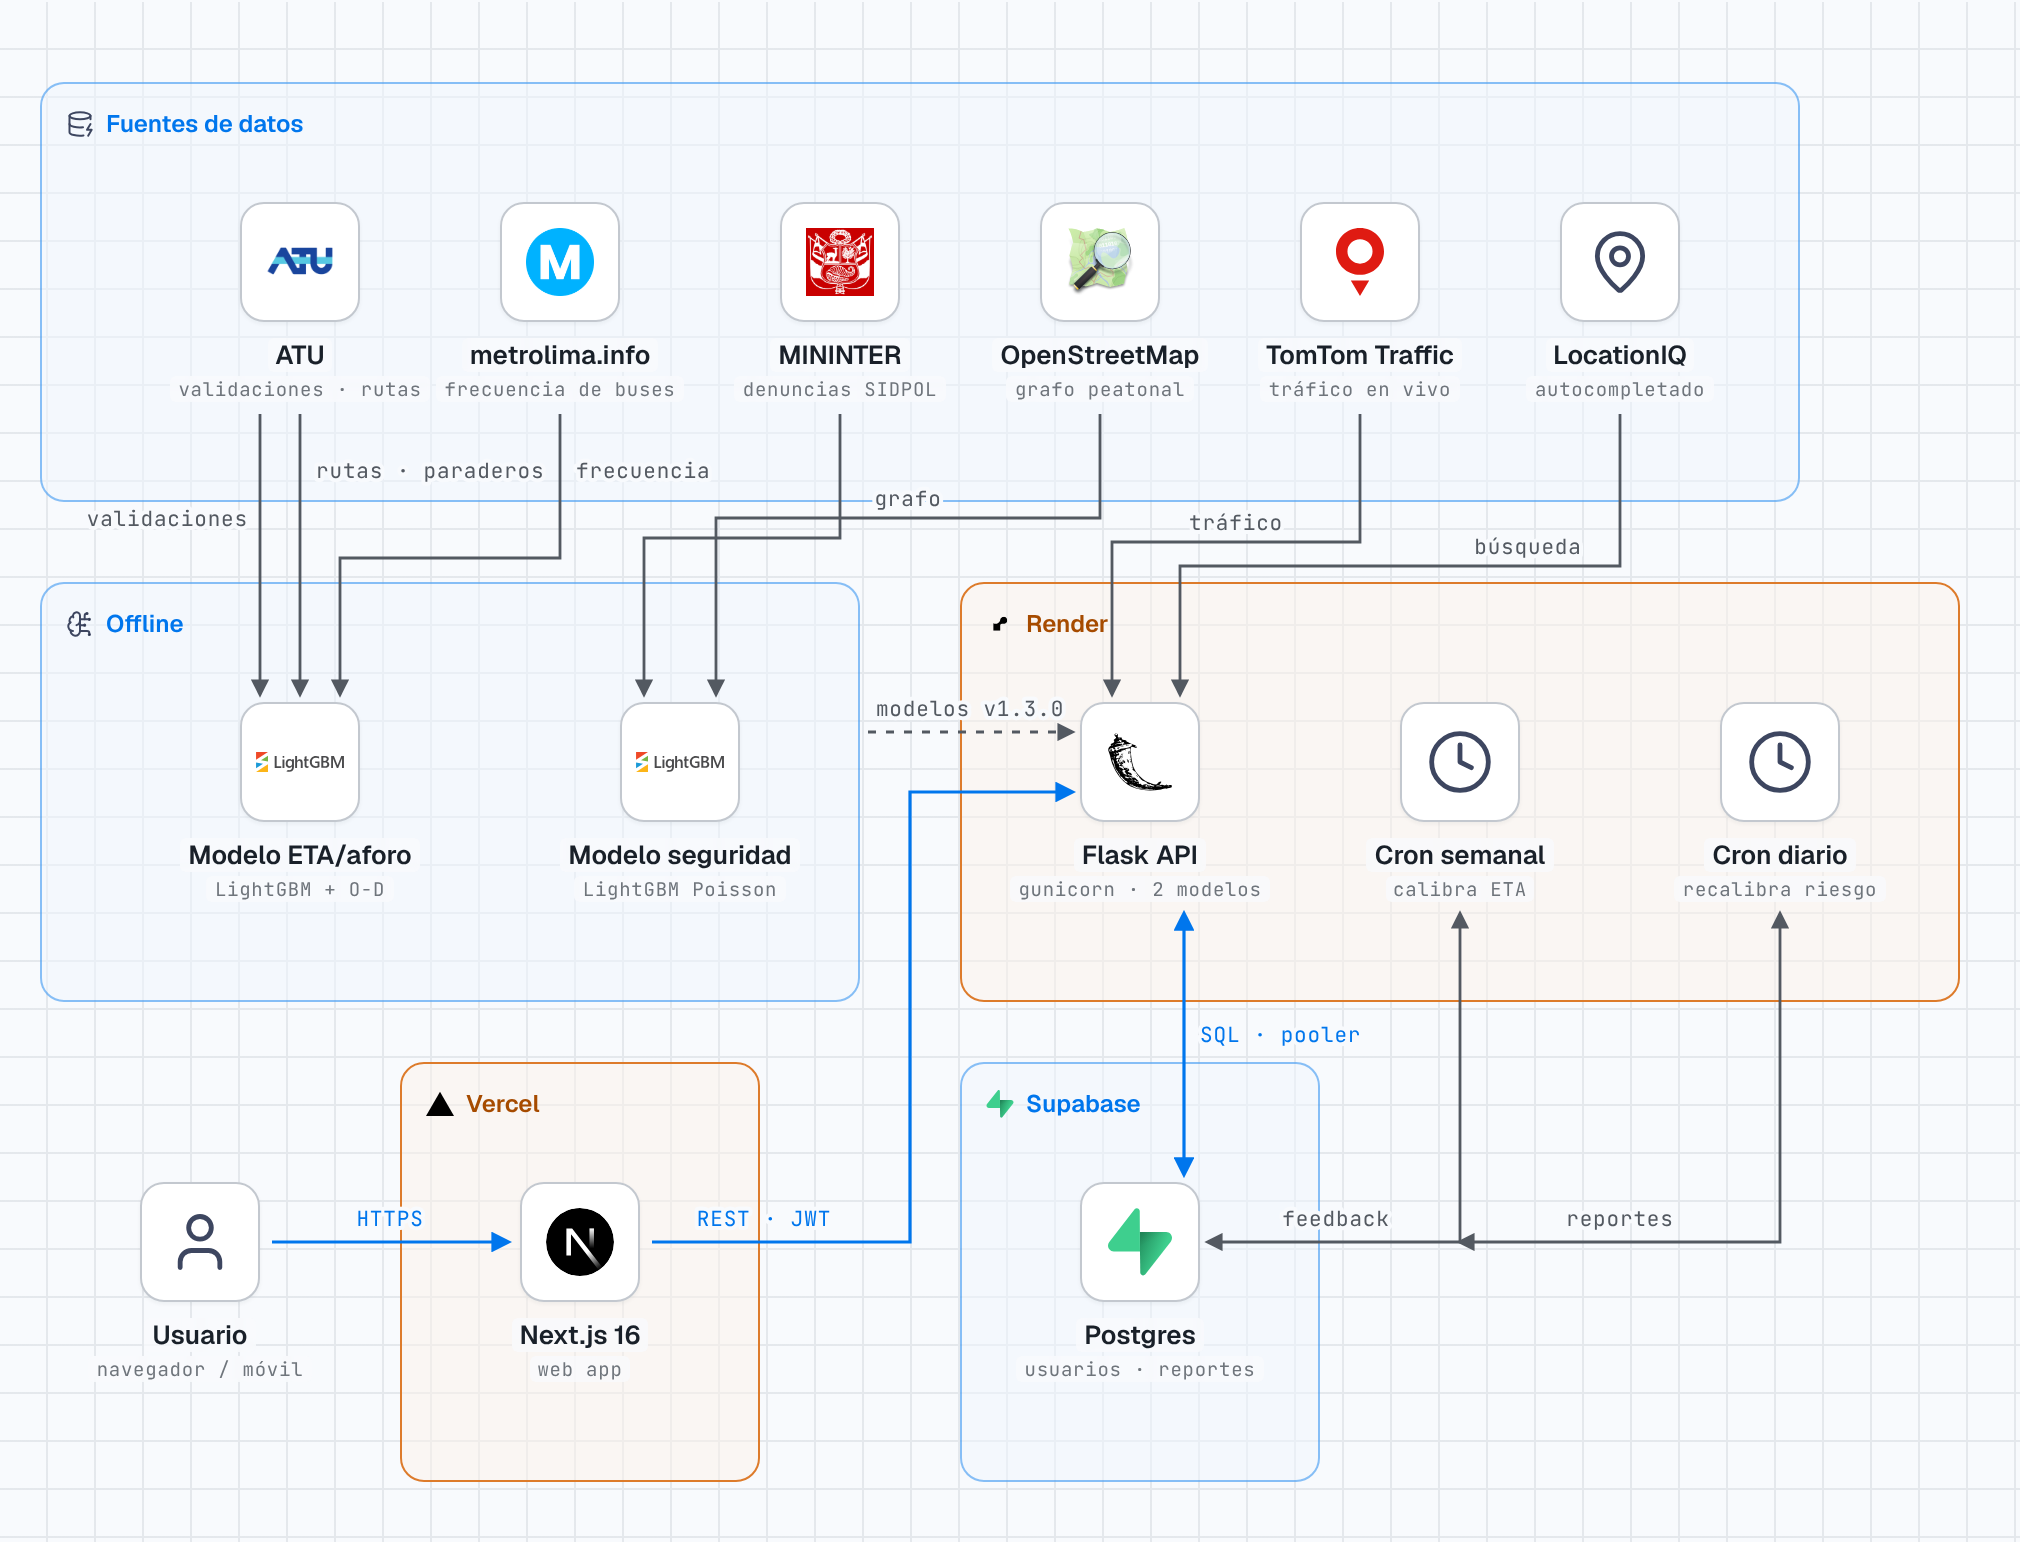
\includegraphics[width=0.92\textwidth]{img/architecture.png}
\caption{Arquitectura. Cuatro fuentes de datos (ATU, MININTER/SIDPOL, OpenStreetMap, TomTom) alimentan dos
modelos separados, entrenados offline: ETA/aforo y seguridad. La API en Render los sirve como artefactos
versionados; la web está en Vercel y la base de datos en Supabase. Dos jobs de Render calibran el ETA
con el feedback de los usuarios y el riesgo con sus reportes.}
\label{fig:arq}
\end{figure}

\begin{itemize}
  \item \textbf{Frontend} (Vercel): Next.js 16 (App Router), React 19, Tailwind 4 y Leaflet;
        paneles de mapa como \emph{bottom sheet} en móvil y tarjeta flotante en escritorio; tema
        claro y oscuro.
  \item \textbf{Backend} (Render, Docker + gunicorn): Flask, SQLAlchemy y JWT. Carga los modelos
        LightGBM y el grafo del Eje 2 en memoria; no necesita una base de datos de demanda.
  \item \textbf{Base de datos} (Supabase, PostgreSQL, vía \emph{pooler}): usuarios, reportes y
        \emph{feedback}. Sin \code{DATABASE\_URL} la API usa SQLite local, solo para desarrollo.
  \item \textbf{Servicios externos} opcionales: TomTom (ajuste de ETA con respaldo al histórico si
        falla) y LocationIQ (autocompletado).
\end{itemize}

\begin{figure}[H]
\centering
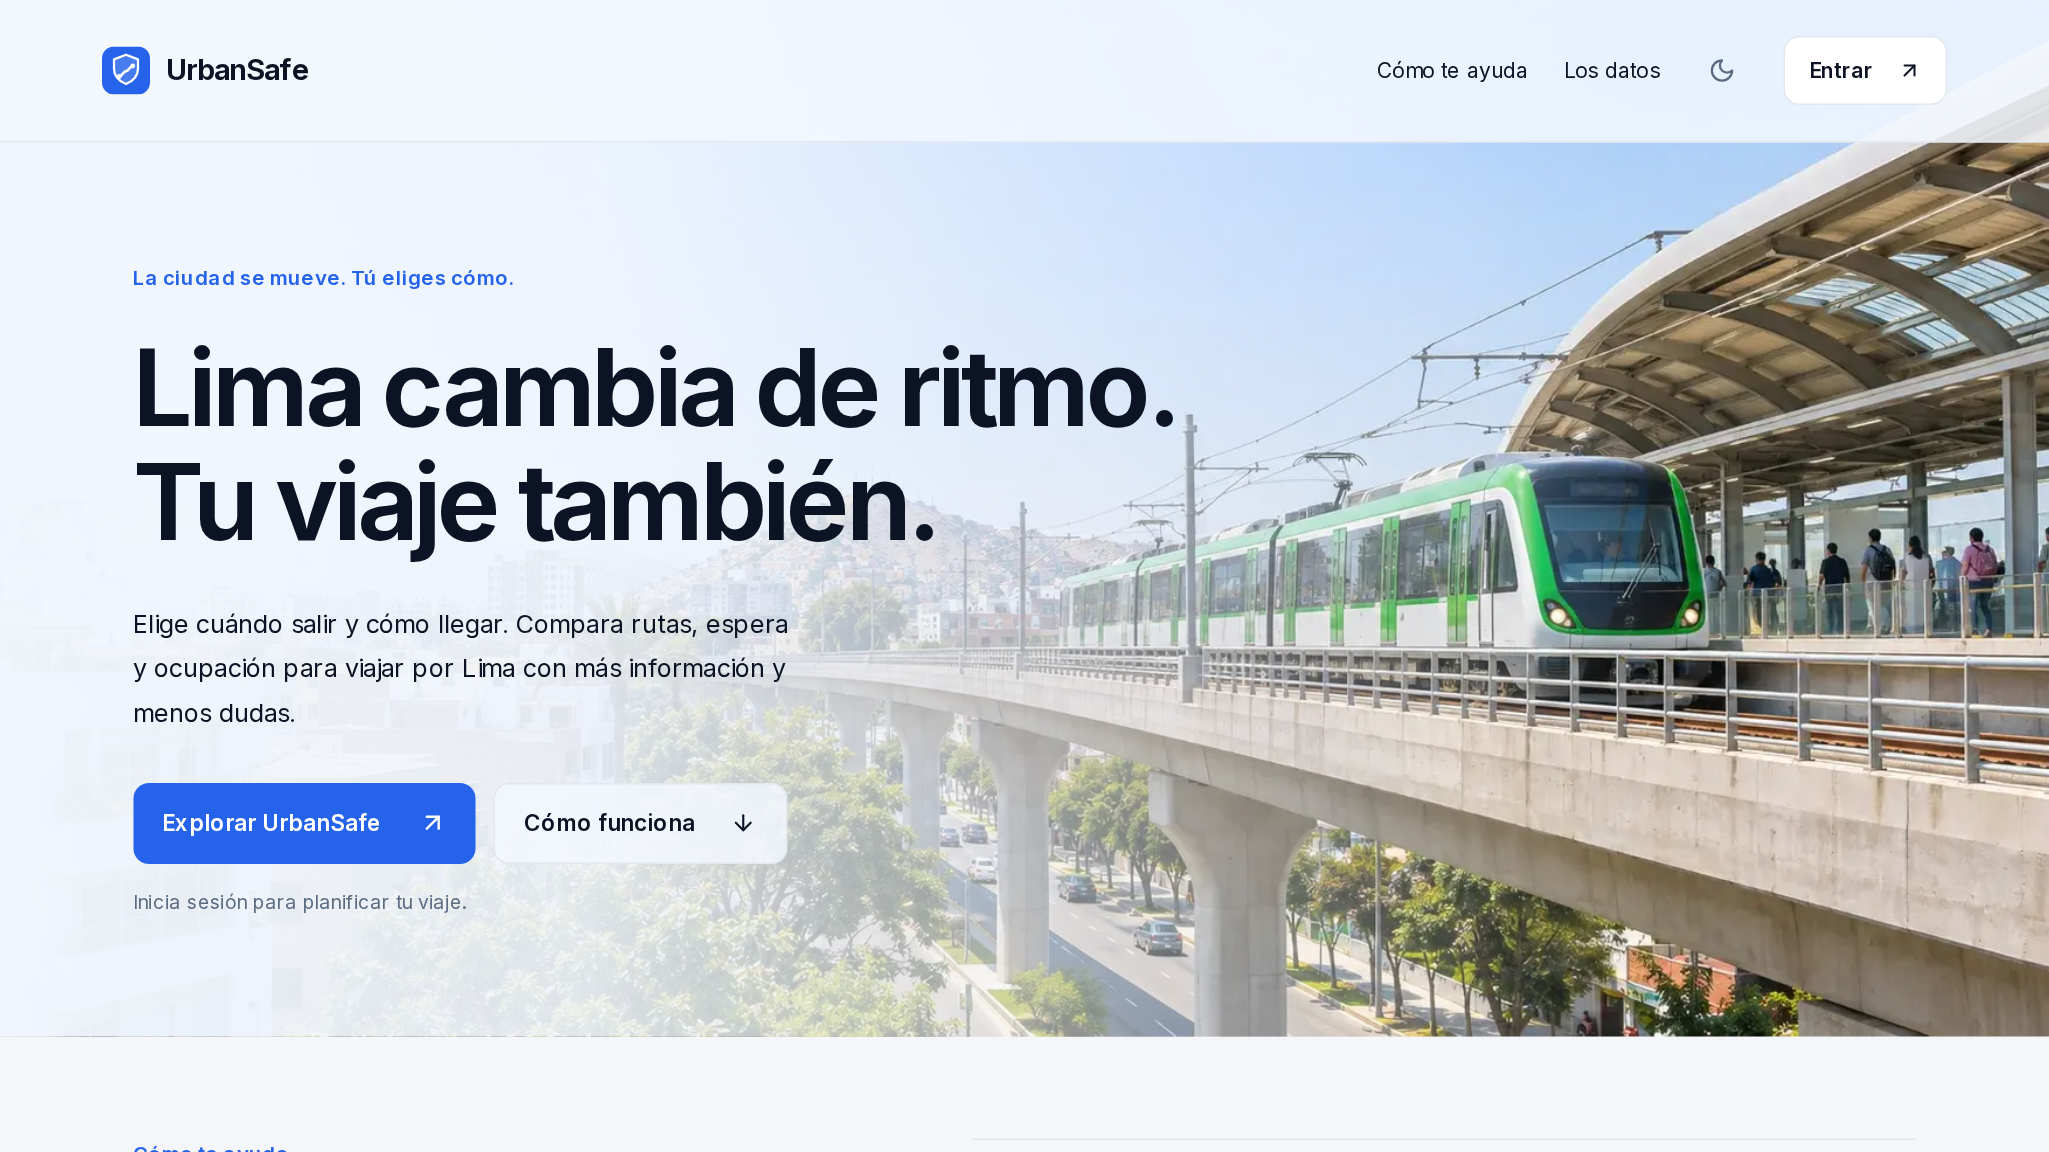
\includegraphics[height=6.2cm]{img/home_web.png}\hspace{0.6cm}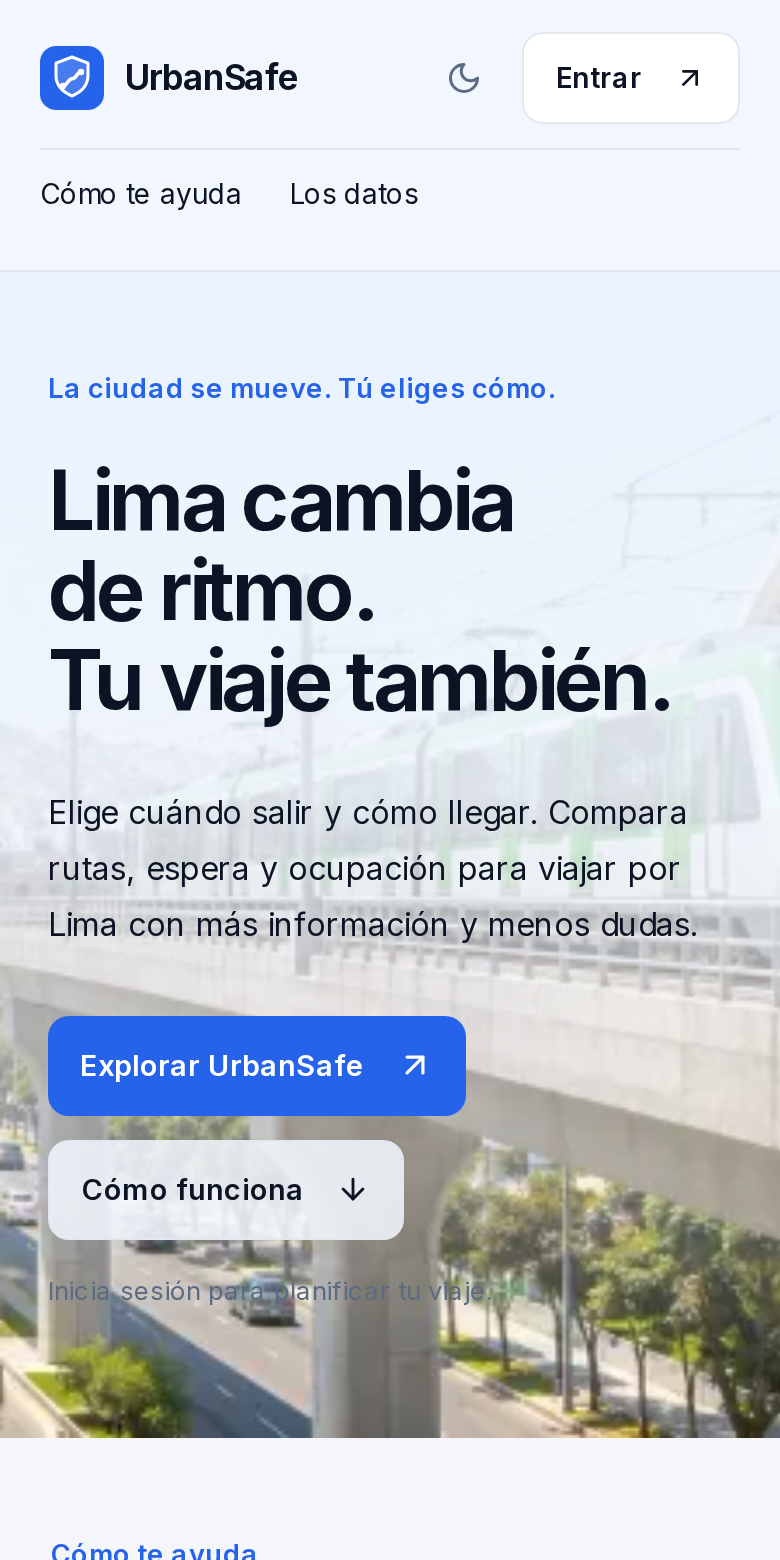
\includegraphics[height=6.2cm]{img/home_mobile.png}
\caption{Página de inicio de la aplicación desplegada: vista web (izquierda) y vista móvil (derecha).}
\end{figure}

\subsection*{Modelos separados y ciclo de aprendizaje}
Los dos modelos son independientes y se entrenan por separado: el de \textbf{ETA/aforo} (LightGBM sobre
validaciones ATU, más la matriz O-D) y el de \textbf{seguridad} (LightGBM Poisson sobre denuncias de
MININTER/SIDPOL y el grafo de OpenStreetMap). En producción solo se carga lo necesario de cada uno.
Después del despliegue hay dos bucles de mejora, ejecutados como Cron Jobs de Render:
\begin{itemize}
  \item \textbf{Semanal (\code{pipeline-semanal}):} calcula métricas con el feedback «Ya abordé» (error del
        ETA mostrado y aforo percibido) y \textbf{recalibra el factor del ETA} con las últimas 8 semanas;
        el ajuste nuevo solo se promueve si mejora al vigente (esquema campeón frente a retador).
  \item \textbf{Diario (\code{pipeline-diario}):} recalibra el riesgo de las calles con los reportes de
        usuarios de los últimos 90 días (acoso, seguimiento, robo) en una tabla de ajustes acotados.
\end{itemize}
\textbf{Importante:} esto es \emph{calibración}, no un re-entrenamiento completo. Los modelos LightGBM
base se vuelven a entrenar offline cuando llegan datos nuevos de la ATU o de SIDPOL, y el feedback de
usuarios todavía no entra como dato de entrenamiento; esa integración queda como trabajo futuro.

\subsection*{Decisiones de diseño relevantes}
\begin{itemize}
  \item \emph{Artefactos versionados en lugar de entrenar en línea}: el plan gratuito de Render
        limita la memoria (512\,MB) y el cómputo.
  \item \emph{Precalcular el grafo peatonal offline}; \code{osmnx} no se usa en producción.
  \item \emph{Declarar el día homólogo} en la respuesta cuando se consulta una fecha sin datos.
\end{itemize}

%======================================================================
\section{Evaluación}

\subsection{Protocolo}

\textbf{Eje 1:} entrenamiento ene--sep 2025, validación 15--31 oct, \textbf{test 1 nov--31 dic}
(61 días) con \emph{rolling-origin}: para cada día de test el modelo solo ve días anteriores y se
reentrena cada 7 días. Una versión intermedia evaluaba con el modelo serializado entrenado con todo
2025 (fuga de información: F1-macro de Metro 0,92 en vez de 0,86); todas las cifras aquí son fuera de
muestra.

\textbf{Eje 2:} entrenamiento $\le$ 2022, validación 2023 (ventanas móviles 2021--2023), \textbf{test
enero--agosto de 2024} evaluado una sola vez con modelos y $\lambda$ ya fijados.

\subsection{Resultados del Eje 1}

\begin{table}[H]
\centering\small
\begin{tabular}{@{}lrrr@{}}
\toprule
\rowcolor{tablehead} \textcolor{white}{\bfseries Sistema} & \textcolor{white}{\bfseries LightGBM} & \textcolor{white}{\bfseries Mejor baseline} & \textcolor{white}{\bfseries Ensemble Chronos} \\
\midrule
Metro L1 & \textbf{0,100} & 0,126 & 0,102 \\
\rowcolor{tablerow} Troncal & \textbf{0,115} & 0,160 & 0,123 \\
Corredores & \textbf{0,113} & 0,167 & 0,120 \\
\rowcolor{tablerow} Alimentadores (ruta$\times$sentido) & \textbf{0,483} & 0,545 & --- \\
\bottomrule
\end{tabular}
\caption{Pronóstico de demanda horaria: WMAPE en test (menor es mejor).}
\end{table}

\begin{table}[H]
\centering\small
\begin{tabular}{@{}lccccc@{}}
\toprule
\rowcolor{tablehead} \textcolor{white}{\bfseries Sistema} & \textcolor{white}{\bfseries Accuracy} & \textcolor{white}{\bfseries F1-macro} & \textcolor{white}{\bfseries WMAPE carga} & \textcolor{white}{\bfseries MAE (pas./veh.)} & \textcolor{white}{\bfseries RNF-01} \\
\midrule
Metro L1 & 0,931 & 0,856 & 0,089 & 40,6 & cumple \\
\rowcolor{tablerow} Troncal & 0,931 & 0,926 & 0,095 & 6,6 & cumple \\
Corredores & 0,919 & 0,655 & 0,196 & 3,9 & F1 no cumple \\
\rowcolor{tablerow} Alimentadores & 0,857 & 0,539 & 0,525 & 5,3 & F1 no cumple \\
\bottomrule
\end{tabular}
\caption{Aforo que ve el usuario (LightGBM + O-D), test fuera de muestra. En todos los sistemas
supera al baseline (media de 4 semanas + O-D); p.\,ej. en el troncal, F1-macro 0,926 frente a 0,899.}
\end{table}

En corredores y alimentadores la clase «Saturado» es rara (1,5\,\% y 2,7\,\% de las horas de test)
y el F1-macro pesa igual a las tres clases; el error de alimentadores está en el reparto horario de
la demanda, muy variable de un día a otro. La banda de incertidumbre del 80\,\% en alimentadores
tiene cobertura empírica de 81,2\,\%.

\subsection{Por qué corredores y alimentadores no cumplen el F1-macro}
\label{sec:f1}
RNF-01 exige dos umbrales a la vez: accuracy $\ge 0{,}75$ y F1-macro $\ge 0{,}72$. En los cuatro sistemas se
cumple la accuracy (0,86 a 0,93); lo que falla en corredores y alimentadores es el F1-macro. Hay tres causas:
\begin{enumerate}
  \item \textbf{La clase «Saturado» es casi inexistente en los buses} (1,5\,\% de las horas de test en corredores y
        2,7\,\% en alimentadores). El F1-macro promedia las tres clases con el mismo peso, por lo que los pocos
        errores en esa clase hunden el promedio aunque el resto vaya bien; la accuracy, dominada por las
        clases frecuentes, apenas se mueve.
  \item \textbf{Menor volumen y más ruido.} Un paradero o una ruta con pocas subidas por hora tiene una demanda
        muy variable de un día a otro. En alimentadores el error del pronóstico es alto (WMAPE 0,48--0,53) porque
        el reparto horario de la demanda cambia mucho; en corredores la carga se reparte entre paraderos
        (WMAPE de la carga 0,196) y el error se acumula.
  \item \textbf{Oferta aproximada.} Las flotas de corredores se derivan con el método del punto de carga máxima y no se
        conocen los buses reales en ruta, por lo que la ocupación (que escala con $1/\text{frecuencia}$) tiene más
        incertidumbre que en Metro L1, que tiene horarios y trenes publicados (el troncal usa una frecuencia publicada, aunque de 2013).
\end{enumerate}
Aun así, el modelo supera al baseline en los cuatro sistemas (por ejemplo, F1-macro de corredores 0,655 frente a
0,555). Los pasos para mejorarlo son agregar covariables de llegadas a la estación de integración (estimadas con
la matriz O-D del troncal), pronosticar por franjas de 2 a 3 horas y, sobre todo, contar con datos más
detallados de la ATU (sección~\ref{sec:refl}).

\textbf{Validación del modelo O-D} (sin bajadas reales): Furness reproduce la Tabla 5.7 de Ortúzar y
Willumsen; en una recuperación sintética el error de bajadas es 0,26 frente a 0,63 del baseline
uniforme; la matriz estimada es 93,5\,\% simétrica; la longitud de la línea (34,7 km) coincide con la
cifra pública (34 km).

\textbf{Recomendación.} La regla inicial decía «abordar» en el 95--99\,\% de las horas. Con costo
generalizado, en 40 viajes de corredores en hora punta la opción anterior estaba en sentido contrario
en el 70\,\% de los casos; la nueva, nunca. Acierto de la recomendación pronosticada frente a la
observada: Metro 99,8\,\%, troncal 96,8\,\%, corredores 99,1\,\%, alimentadores 97,7\,\% (AC-03).

\subsection{Resultados del Eje 2}

\begin{table}[H]
\centering\small
\begin{tabular}{@{}lccccc@{}}
\toprule
\rowcolor{tablehead} \textcolor{white}{\bfseries Modelo (test 2024)} & \textcolor{white}{\bfseries Deviance} & \textcolor{white}{\bfseries MAE} & \textcolor{white}{\bfseries Spearman} & \textcolor{white}{\bfseries Top 5\,\%} & \textcolor{white}{\bfseries Top 10\,\%} \\
\midrule
B0 constante & 2,292 & 0,485 & --- & 3,6\,\% & 8,3\,\% \\
\rowcolor{tablerow} B1 historial del segmento & 0,988 & 0,313 & 0,460 & 67,1\,\% & 78,5\,\% \\
B2 Empirical Bayes & 0,992 & 0,408 & 0,362 & 61,7\,\% & 72,9\,\% \\
\rowcolor{tablerow} M1 GLM Poisson & 0,768 & 0,354 & 0,394 & 67,5\,\% & 78,2\,\% \\
\textbf{M2 LightGBM Poisson} & \textbf{0,701} & 0,329 & 0,407 & \textbf{70,2\,\%} & \textbf{80,3\,\%} \\
\bottomrule
\end{tabular}
\caption{Riesgo por segmento, test enero--agosto de 2024. «Top $k$\,\%» es la fracción de eventos que
cae en el $k$\,\% de calles marcadas como más riesgosas.}
\end{table}

LightGBM tiene la menor deviance (29\,\% menos que el historial) y gana en las tres ventanas móviles
de validación (figura~\ref{fig:vm}). El historial ordena ligeramente mejor el conjunto completo
(Spearman 0,460 frente a 0,407), por lo que el ordenamiento global es modesto: lo sólido es evitar
las calles con más denuncias \emph{en promedio}, no afirmar que una calle concreta es segura.

\begin{figure}[H]
\centering
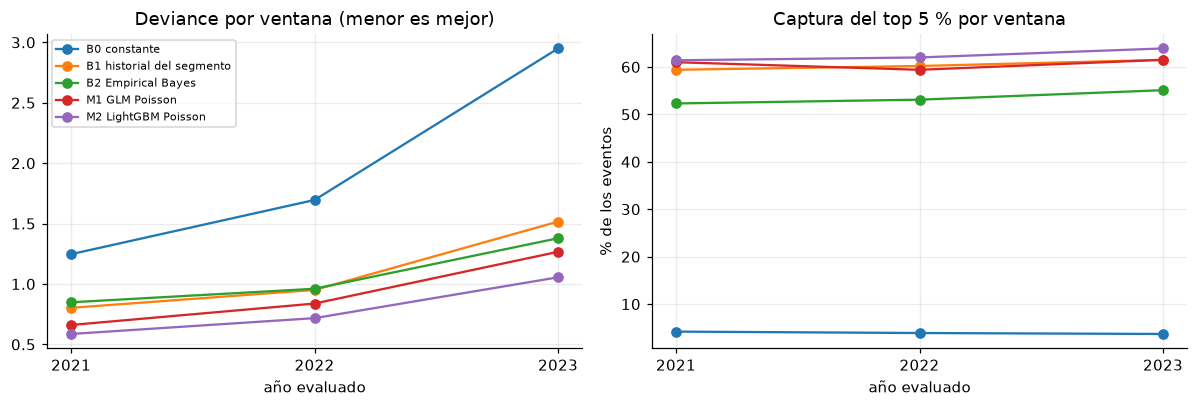
\includegraphics[width=0.85\textwidth]{img/modelo_ventanas_moviles.png}
\caption{Deviance de Poisson en las ventanas móviles 2021--2023.}
\label{fig:vm}
\end{figure}

\begin{figure}[H]
\centering
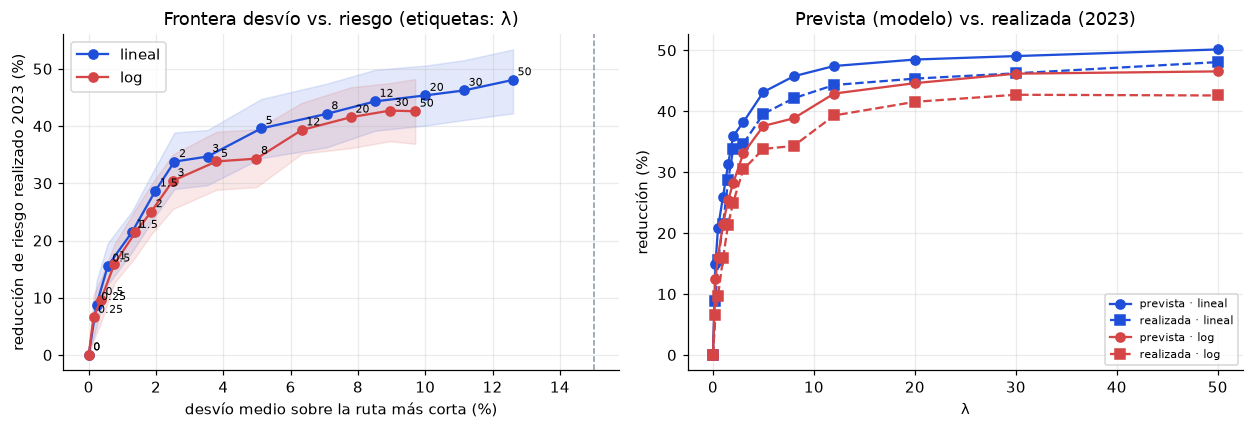
\includegraphics[width=0.85\textwidth]{img/ruteo_frontera_lambda.png}
\caption{Frontera desvío frente a reducción de riesgo para distintos $\lambda$; se eligió
$\lambda=12$ (rendimientos decrecientes después).}
\end{figure}

\textbf{Confirmación en el test ($\lambda=12$, medida una sola vez):} desvío medio 8,7\,\% (p90
22,6\,\%) y reducción realizada de denuncias de \textbf{43,8\,\%} (IC 95\,\% 38,6--50,2). De noche,
desvío 10,4\,\% y 50,6\,\% menos. Por tipo de acceso: alimentador 70,3\,\%, troncal 47,2\,\%,
corredor 45,1\,\% y Metro 27,6\,\%.

\subsection{Casos de estudio}

\paragraph{Caso 1: regreso desde Gamarra (Eje 1).} Una usuaria que vive en Villa El Salvador abre la
app en la estación Gamarra el miércoles 4 de noviembre de 2026 a las 18:00 y elige su destino. Como
no hay datos ATU de 2026, el backend usa el día homólogo (5-11-2025) y lo declara. Respuesta de la
API:

\begin{center}\small
\begin{tabular}{@{}lccccl@{}}
\toprule
\rowcolor{tablehead} \textcolor{white}{\bfseries Sentido} & \textcolor{white}{\bfseries Clase} & \textcolor{white}{\bfseries Ocupación} & \textcolor{white}{\bfseries A bordo} & \textcolor{white}{\bfseries Espera} & \textcolor{white}{\bfseries Recomendación} \\
\midrule
hacia Villa El Salvador & De pie & 48\,\% & $\approx$576 & 1,5 min & Abordar \\
\rowcolor{tablerow} hacia Bayóvar & Saturado & 85\,\% & $\approx$1014 & 1,5 min & Abordar (a las 19:00 sigue saturado) \\
\bottomrule
\end{tabular}
\end{center}

En su sentido el tren va de pie pero sin saturar; el sentido contrario (regreso a San Juan de
Lurigancho) va saturado. La versión 1 no distinguía sentidos y habría mostrado el mismo valor para
ambos.

\paragraph{Caso 2: hora punta en el troncal.} En Naranjal a las 7:00 hacia el centro la ocupación
estimada es 110\,\% («Saturado») y la app recomienda \emph{esperar el siguiente}, porque la hora
siguiente es menos crítica.

\paragraph{Caso 3: último tramo a pie (Eje 2).} Para un trayecto de 627 m (mediana de la ruta más
corta en la evaluación) con $\lambda=12$, la ruta segura camina en promedio un 8,7\,\% más y evita
alrededor del 44\,\% de las denuncias registradas en las calles recorridas. La app muestra siempre la
ruta más corta como alternativa y no un «porcentaje de seguridad» de calles individuales.

\subsection{Pruebas}
El backend incluye 217 pruebas automáticas (\code{pytest}): algoritmo de Furness, calendario,
API, recomendación, latencia P95, recarga de modelos y Eje 2 (ruteo, recalibración). Se complementan
con \code{npx tsc --noEmit} y \code{next build} en el frontend.

%======================================================================
\section{Limitaciones, ética y riesgos}
\label{sec:limit}

\begin{itemize}
  \item \textbf{Sin bajadas ni GPS:} la matriz O-D se valida de forma sintética y contra cifras
        públicas, no contra viajes reales.
  \item \textbf{Datos 2025:} las fechas de 2026 usan el día homólogo; no capturan cambios de flota ni
        aperturas posteriores. La oferta del troncal usa un dato de 2013 (117 buses/h en punta).
  \item \textbf{Corredores y alimentadores} no cumplen el F1-macro de RNF-01. Próximos pasos:
        covariables de llegadas a la estación de integración y pronóstico por franjas de 2--3 horas.
  \item \textbf{Denuncias no son delito:} subregistro (muy alto en acoso y violencia sexual) y sesgo
        de quién denuncia y dónde se registra. Los alimentadores salen «muy seguros» sobre todo por
        menor registro y coordenadas en zonas periféricas; no es un indicador de menor delito.
  \item \textbf{Cobertura desigual} de coordenadas entre comisarías y años; se corrige con
        ponderación bajo el supuesto MAR, que no es verificable. 52\,\% de los eventos cae fuera de
        las zonas de 10 minutos, y los datos desde septiembre de 2024 no se usan.
  \item \textbf{El nivel absoluto de eventos no se predice bien} (previsto/observado de 0,56 a 0,65 en
        validación y 1,11 en test): el modelo sirve para ordenar, no para contar.
  \item \textbf{Despliegue gratuito:} el primer pedido tras inactividad tarda $\sim$50 s.
\end{itemize}

\textbf{Reglas éticas del producto:} nunca se exponen reportes individuales ni usuarios; el botón de
alerta ofrece llamar al 105; se declara el subregistro y el sesgo social; y no se penaliza ninguna
zona por la «calidad de vida» del barrio.

%======================================================================
\section{Conclusiones y trabajo futuro}

UrbanSafe AI integra, de extremo a extremo, un pronóstico de aforo explicable y una ruta peatonal
informada por denuncias, con evaluación fuera de muestra, baselines y limitaciones declaradas. El
Eje 1 cumple los requisitos de exactitud en Metro L1 y troncal; el Eje 2 reduce el riesgo realizado
en torno a 44\,\% con un desvío moderado.

\textbf{Trabajo futuro:}
\begin{enumerate}
  \item Mejorar el F1-macro de corredores y alimentadores.
  \item Integrar el feedback y los reportes de usuarios al entrenamiento (y no solo a la calibración), incluido el aforo percibido.
  \item Actualizar el riesgo con datos recientes de denuncias y un geocodificador local.
  \item Ampliar las pruebas con usuarios reales a una muestra mayor y con encuesta formal (AC-06); la primera prueba de campo ya aportó correcciones.
  \item Infraestructura sin suspensión para cumplir la disponibilidad de RNF-03.
\end{enumerate}

%======================================================================
\section{Declaración de contribución}



\begin{table}[H]
\centering\small
\begin{tabularx}{\textwidth}{@{}>{\raggedright\arraybackslash}p{4.4cm}X@{}}
\toprule
\rowcolor{tablehead} \textcolor{white}{\bfseries Integrante} & \textcolor{white}{\bfseries Contribuciones principales} \\
\midrule
\textbf{Elmer Villegas}\newline\textit{Data Engineer y full stack} &
\begin{itemize}[nosep,leftmargin=1em]
  \item Ingesta de datos, pipelines y diccionarios de datos.
  \item Infraestructura y despliegue (Vercel, Render, Supabase, Docker).
  \item Eje 2: denuncias, riesgo por calle y ruteo seguro.
  \item Desarrollo full stack, junto con Alessandro, y documentación.
\end{itemize} \\
\rowcolor{tablerow} \textbf{Alessandro Monzón}\newline\textit{Product Manager, AI/ML y full stack} &
\begin{itemize}[nosep,leftmargin=1em]
  \item Requerimientos y gestión del producto.
  \item Backend y frontend, junto con Elmer.
\end{itemize} \\
\textbf{Juan Velo}\newline\textit{Data Scientist} &
\begin{itemize}[nosep,leftmargin=1em]
  \item Eje 1: modelado, explicabilidad y evaluación.
  \item Pronóstico de demanda y aforo, y matriz origen-destino.
\end{itemize} \\
\bottomrule
\end{tabularx}
\caption{Reparto del trabajo.}
\end{table}

%======================================================================
\section{Reflexión sobre el proceso de desarrollo}
\label{sec:refl}

\begin{itemize}
  \item \textbf{Qué funcionó:} dividir el producto en dos ejes con criterios de aceptación medibles; fijar las
        reglas de decisión antes de mirar el test; detectar y corregir la fuga de información en la evaluación;
        repartir el trabajo por roles (datos, producto/full stack, modelado); y llevar el plan con hitos (\emph{milestones}) e \emph{issues} en GitHub, que ordenó las entregas semanales.
  \item \textbf{Retos:} datos de la ATU solo con subidas; cobertura desigual de coordenadas en las denuncias;
        límites de memoria del plan gratuito de Render; coordinar un equipo pequeño con tres frentes a la vez.
  \item \textbf{Qué cambiaríamos:}
    \begin{itemize}
      \item \emph{Conocer mejor el dataset de la ATU al inicio.} No estamos seguros de si la base de validaciones
            trae el identificador de la tarjeta; nos faltó contexto para pedir un conjunto de datos mejor. Con ese
            identificador se podrían reconstruir los viajes y las bajadas en lugar de estimarlas.
      \item \emph{Probar antes con usuarios reales.} Una prueba de campo (un integrante usó la app en sus trayectos del
            trabajo a la universidad y de regreso) detectó un error que las pruebas automáticas no vieron: la
            recomendación siempre sugería corredores, incluso estando en una estación. Se corrigió, pero con pruebas de
            campo desde antes, y con más usuarios, lo habríamos encontrado antes.
      \item \emph{Decidir antes la plataforma.} Empezamos pensando en un APK, pero desplegarlo para todos los
            dispositivos resultó difícil y optamos por una web responsive. Quizá sin ese tiempo gastado habríamos
            mejorado el modelo.
      \item \emph{Planificar un despliegue sin suspensión.} El plan gratuito de Render duerme el servicio y la primera
            consulta tarda unos 50 segundos.
    \end{itemize}
  \item \textbf{Lecciones para futuros proyectos:}
    \begin{itemize}
      \item El modelo de aforo puede mejorar con el identificador de la tarjeta, y más aún trabajando de la mano con
            la ATU: el Metropolitano y su troncal sí cuentan con GPS para ver los buses en tiempo real, y con
            cámaras en algunas unidades se podría usar visión por computador para contar pasajeros con más precisión.
      \item En seguridad usamos denuncias, que no son necesariamente delitos. Algunas no traían la dirección del
            hecho sino la de la comisaría, y hay personas que no denuncian en ciertas calles, lo que sesga el riesgo
            hacia las zonas donde sí se denuncia. Por eso el producto muestra tendencias y no garantías.
      \item Documentar desde el inicio las limitaciones de los datos y comunicarlas en la interfaz evita
            promesas que el modelo no puede cumplir.
      \item Un producto de datos necesita medir su desempeño en uso real (feedback y reportes) para poder
            calibrarse, no solo evaluarse sobre datos históricos.
    \end{itemize}
\end{itemize}

%======================================================================
\section*{Referencias}
\addcontentsline{toc}{section}{Referencias}
\begin{itemize}[leftmargin=1.2em]
  \item Ortúzar, J. de D. y Willumsen, L. G. \emph{Modelos de Transporte}. Furness, gravedad,
        estimación de matrices O-D y costo generalizado.
  \item Galbrun, E., Pelechrinis, K. y Terzi, E. (2016). Urban navigation beyond shortest route: the
        case of safe paths. \emph{Information Systems} 57.
  \item Whelan, G. y Crockett, J. Multiplicadores de hacinamiento en el valor del tiempo de viaje.
  \item INEI (2025). \emph{Percepción de la Inseguridad Ciudadana y Victimización en Áreas Urbanas de
        Lima Metropolitana}.
  \item ProTransporte y ATU. Portal de Datos Abiertos. \url{https://sistemas.protransporte.gob.pe/DatosAbiertos/}
  \item Ke, G. et al. LightGBM. \url{https://github.com/microsoft/LightGBM}
\end{itemize}

\clearpage
\begin{landscape}
\thispagestyle{empty}
\section*{Anexo A. Data Product Canvas final}
\addcontentsline{toc}{section}{Anexo A. Data Product Canvas final}
\label{anx:canvas}
\centering
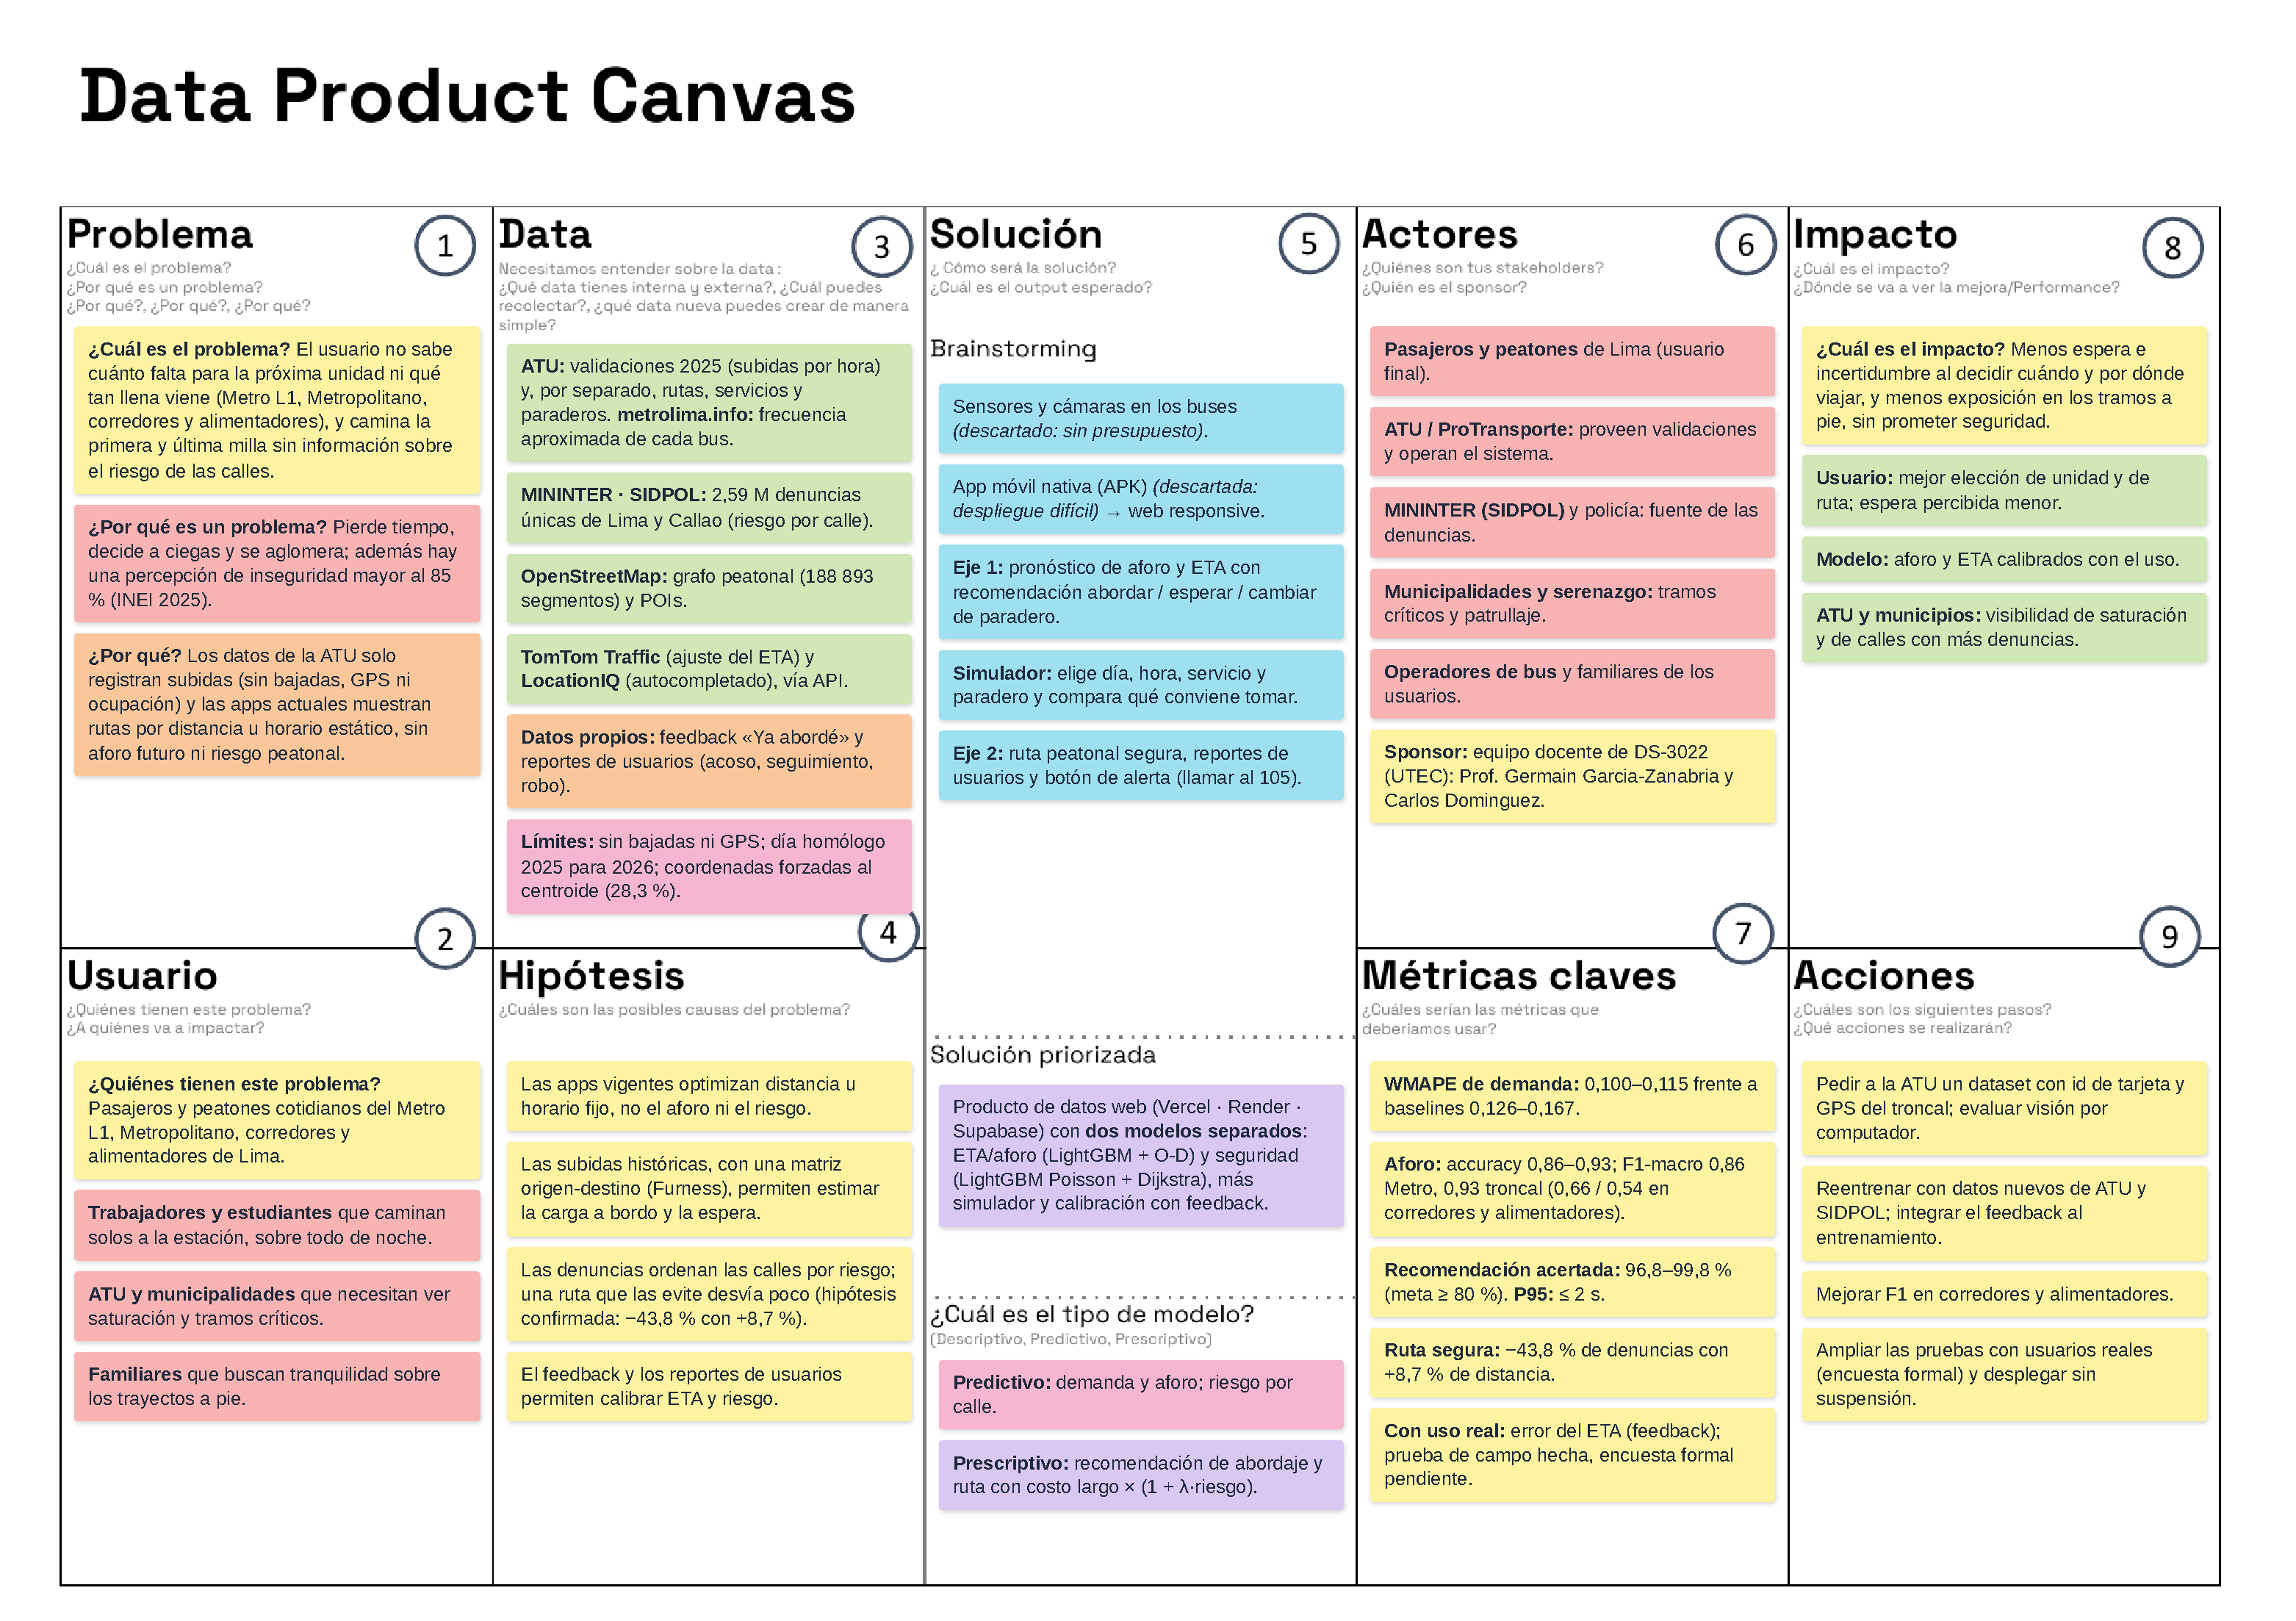
\includegraphics[width=\linewidth,height=0.72\textheight,keepaspectratio]{img/DataProductCanvas.pdf}

\captionof{figure}{Data Product Canvas final de UrbanSafe AI (plantilla del curso).}
\end{landscape}

\end{document}
